\documentclass[a4paper,12pt,twoside,openany]{report}

\usepackage{polski}
\usepackage{helvet}
\usepackage[T1]{fontenc}
\usepackage{anyfontsize}
\usepackage[utf8]{inputenc}
\usepackage[pdftex]{graphicx}
\usepackage{tabularx}
\usepackage{array}
\usepackage[polish]{babel}
\usepackage{subfigure}
\usepackage{amsfonts}
\usepackage{verbatim}
\usepackage{indentfirst}
\usepackage[pdftex]{hyperref}
\usepackage{amsmath}
\usepackage{float}
\usepackage{subfigure}

\usepackage{enumitem}% http://ctan.org/pkg/enumitem
\setlist[itemize]{noitemsep, topsep=0pt}

\newcommand{\ImgPath}{.}
\newcommand{\TODO}{\textbf{TODO}}
\newcommand{\tech}{\texttt}

\def\oprawa{1.05cm}
\addtolength{\oddsidemargin}{\oprawa}
\addtolength{\evensidemargin}{-\oprawa}

\usepackage{multirow}
\usepackage{enumitem}	
\setlist{listparindent=\parindent, parsep=\parskip} 

\usepackage{prmag2017} 

\title{Rozpoznawanie gestów na przykładzie gry papier, kamień, nożyce}

\author{Adrian Szewczyk}
\nrindeksu{279074}

\opiekun{mgr inż. Marek Wdowiak}
\terminwykonania{1 lutego 2018} 
\rok{2018}


\opinie{
  \input{opiniaopiekuna.tex}
  \newpage
  \newpage
\begin{center}
 {\large\bf  Recenzja } \\
pracy dyplomowej magisterskiej wykonanej przez dyplomanta\\
{\bf Zdolnego Studenta i Pracowitego Kolegę} \\
 Wydział Elektryczny, kierunek Informatyka,  Politechnika Warszawska\\
Temat pracy\\
\textit{\bf
TYTUŁ PRACY DYPLOMOWEJ
}\\
\end{center}
\medskip
\noindent
Recenzent: {\bf prof. nzw. dr hab. inż. Jan Surowy}\\
Ocena pracy dyplomowej: {\bf bardzo dobry}
\medskip


\centerline{\bf Treść recenzji}
   Celem pracy dyplomowej panów dolnego Studenta i Pracowitego Kolegi  było
opracowanie systemu pozwalającego symulować  i opartego o oprogramowanie o
otwartych źródłach (ang. Open Source). Jak piszą Dyplomanci, starali się opracować
system, który łatwo będzie dostosować do zmieniających się dynamicznie wymagań,
będzie miał niewielkie wymagania sprzętowe i umożliwiał dalszą łatwą rozbudowę oraz
dostosowanie go do potrzeb.
Przedstawiona do recenzji praca składa się z krótkiego wstępu jasno i
wyczerpująco opisującego oraz uzasadniającego cel pracy, trzech rozdziałów (2-4)
zawierających bardzo solidny i przejrzysty opis: istniejących podobnych
rozwiązań (rozdz. 2), komponentów rozpatrywanychjako kandydaci do
tworzonego systemu (rozdz. 3) i wreszcie zagadnień wydajności wirtualnych
rozwiązań, zwłaszcza w kontekście współpracy  kilku elementów
 sieci (rozdział 4). Piąty rozdział to opis przygotowanego przez
Dyplomantów środowiska obejmujący opis konfiguracji
środowiska oraz przykładowe ćwiczenia laboratoryjne (5 ćwiczeń). Ostatni, szósty
rozdział pracy to krótkie zakończenie, które wylicza także możliwości dalszego
rozwoju projektu. W ramach przygotowania pracy Dyplomanci zebrali i przedstawili w
bardzo przejrzysty sposób duży zasób informacji o narzędziach, Rozdziały 2, 3 i 4 świadczą o dobrej orientacji
w nowoczesnej i ciągle intensywnie rozwijanej tematyce stanowiącej
zakres pracy i o umiejętności syntetycznego, przejrzystego przedstawienia tych
wyników. Drobne  mankamenty tej części pracy to zbyt skrótowe omawianie
niektórych zagadnień technicznych, zakładające dużą początkową wiedzę czytelnika
i dość niestaranne podejście do powołań na źródła.
Utrudnia to w pewnym stopniu czytanie pracy i zmniejsza jej wartość dydaktyczną
(a ta zdaje się być jednym z celów Autorów), ale jest zrekompensowane zawartością
merytoryczną. Praca zawiera dwa dodatki, z których pierwszy obejmuje wyniki
eksperymentów i badań nad wydajnością, a drugi to źródła
skryptów budujących środowisko. Praca
zawiera niestety dość dużą liczbę drobnych błędów redakcyjnych, ale nie wpływają
one w sposób istotny na na jej czytelność i wartość. W całej pracy przewijają
się samodzielne, zdecydowane wnioski Autorów, które są wynikiem własnych i
oryginalnych badań.  Rozdział 5 i dodatki pracy przekonują mnie, że Dyplomanci dość
dobrze zrealizowali postawione przed nimi zadanie. Pozwala to stwierdzić, że
wykazali się więc także umiejętnością zastosowania w praktyce wiedzy
przedstawionej w rozdziałach 2-4. Kończący pracę rozdział szósty świadczy o
dużym (ale moim zdaniem uzasadnionym) poczuciu własnej wartości i jest
świadectwem własnego, oryginalnego spojrzenia na tematykę przedstawioną w pracy
dyplomowej. Uważam, że cele postawione w założeniach pracy zostały pomyślnie
zrealizowane. Proponuję ocenę bardzo dobrą (5).

\vskip 1cm
{
\raggedleft
(data, podpis)\kern1cm

}
}

\streszczenia{
  \newpage
\begin{center}
\large \bf
Rozpoznawanie gestów na przykładzie gry papier, kamień, nożyce
\end{center}

\section*{Streszczenie}
W pracy inżynierskiej zostało przedstawione podejście do problemu rozpoznawania gestów przez wszystkie jego etapy. W pierwszym etapie został przedstawiony zakres i cel pracy. Kolejne dwa rozdziały to teoretyczny wstęp do zagadnień oraz wykorzystanych narzędzi w pracy. 

Rozdział ,,rozwiązywanie problemu'' pokazuje podejście do klasyfikacji gestów na przykładzie gry papier, kamień, nożyce. Obrazuje aktywizację oraz  przetwarzanie danych w celu uzyskania jak najlepszego zbioru danych. W późniejszej części zostały opisane etapy filtracji, segmentacji dłoni. Po uzyskaniu zbioru danych zostały stworzone klasyfikatory. Pierwszym podejściem było stworzenie klasyfikatora KNN, a następnie stworzenie klasyfikatora bazującego na sieciach neuronowych. 

Zakończenie pracy to podsumowanie wykonanej pracy, porównanie wyników uzyskanych przez użyte klasyfikatory oraz opisanie wniosków zaobserwowanych podczas wykonywania pracy inżynierskiej.

\bigskip
{\noindent\bf Słowa kluczowe:} rozpoznawanie gestów, klasyfikacja, sieci neuronowe, OpenCV, TensorFlow, Keras, klasyfikator KNN

\vskip 2cm


\begin{center}
\large \bf
ENG Rozpoznawanie gestów na przykładzie gry papier, kamień, nożyce
\end{center}

\section*{Abstract}

\bigskip
{\noindent\bf Keywords:} ENG rozpoznawanie gestów, klasyfikacja, python, sieci neuronowe

\vfill
}

\begin{document}
\maketitle


\chapter{Wstęp}
\section{Wprowadzenie}
Gesty są jednym z najważniejszych elementów komunikacja pomiędzy ludźmi. Niewerbowana mowa może przekazać zdecydowanie więcej informacji niż tylko słowa wypowiedziane przez nadawcę. Gesty mogę, również zastąpić słowa i być wykorzystywane jako zamiennik na słyszalne słowa. Przykładem tego jest język migowy, który pozwala na wzajemną komunikację ludzi głuchych . Oprócz samej mowy gesty, mają też inne zastosowania. Przykładem takim może być gra papier, kamień, nożyce. W której każdy z graczy pokazuje jeden z trzech dostępnym gestów. I w zależności od kombinacji gestów pokazanych przez graczy określany jest zwycięzca.

Klasyfikacja gestów jest powszechnym problem przetwarzania obrazów. Jest to temat obszerny i coraz lepiej zbadanym problem nauki. Klasyfikacja gestów ma szerokie zastosowanie. Jedną zalet rozpoznawania gestów jest możliwość sterowania naszym smartfonem za pomocą ruchu rąk. Po wykonaniu gestu a następnie po rozpoznaniu go przez  oprogramowanie telefonu wykonywana jest określona akcja. Innym wykorzystaniem klasyfikacji gestów jest sterowanie gier, podając jako przykład konsolę Nintendo Wii.

\section{Cel pracy}
W swojej pracy dyplomowej będę chciał przedstawić sposób podejścia do problemu klasyfikacji gestów, a następnie zaimplementować działające rozwiązanie i wykorzystać go w praktyce, na przykładzie gry papier, kamień, nożyce. Stworzona gra pozwoli na automatyczne rozpoznawanie gestów, liczenie punktów i byciem arbitrem w grze. Wszystkim tym zajmie się specjalnie napisany system, który będę chciał zaprezentować w tej pracy dyplomowej.

\chapter{Przetwarzanie obrazów}
\section{Cyfrowe przetwarzanie obrazów binarnych}
Cyfrowe przetwarzanie obrazów binarnych jest to dziedzina przetwarzania obrazów cyfrowych zajmująca się algorytmami obróbki obrazów binarnych. 

\begin{figure}[H]	
	\centering
	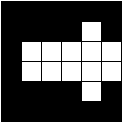
\includegraphics[width=0.7\textwidth]{\ImgPath/rys/bin.png}
	
	\caption{  \textbf{Przykładowy obraz binarny}}
\end{figure}

Obrazy binarne składają się z pikseli, które mogą przyjmować jedynie dwie wartości. Piksele takie możmy oznaczać różnymi symboli, np. 0/1, false/true czy też (0,0,0)/(255,255,255). Podczas interpretacji obrazu jedne z pikseli można traktować jako tło, inne zaś jako część obiektu. Dzięki czemu jesteśmy wstanie rozróżnić interesującą nas część obrazu od pozostałej części. 

\section{OpenCV}
OpenCV (Open Source Computer Vision Library) jest to otwartoźródłowa biblioteka wykorzystywana przy rozpoznawaniu obrazów oraz przy uczeniu maszynowym. Została napisana w języku C przez programistów z firmy Intel w 1999 roku.

W późniejszym czasie kolejne części biblioteki były także pisane w języku C++. OpenCV umożliwia pisanie kodów nie tylko w językach C i C++ ale również mamy możliwość wykorzystywania tej biblioteki w językach Python, Java czy też Matlab. Co więcej zostały udostępnione nakładki do języków takich jak C\#, Perl, Ruby czy Haskell aby móc również wykorzystywać zalety  biblioteki. 

OpenCV udostępnia zaawansowaną funkcjonalność  w szeroko rozumianym pojęciu rozpoznawaniu obrazów:

\begin{itemize}
	\item przetwarzania obrazów
	\item klasyfikowaniu wzorców
	\item dokładnych pomiarów obrazów
\end{itemize}

Jako główne zalety OpenCV możemy wyróżnić, że jest on darmowy oraz otwartoźródłowy. Zawiera bogaty zakres funkcjonalności, a kod biblioteki został napisany w sposób zoptymalizowanym, tak aby operacje wymagające dużej mocy obliczeniowej czy działające w czasie rzeczywistym mogły wykonywać się możliwie jak najszybciej.

OpenCV znalazło zastosowanie w wielu dziedzinach naszego codziennego życia:
\begin{itemize} 
	\item medycyna
	\item robotyka
	\item samochody autonomiczne
	\item systemy antywłamaniowe 
	\item systemy zabezpieczające
	\item rozpoznawanie gestów
	\item segmentacja obiektów
	\item wykrywanie ruchu
	\item rozszerzona rzeczywistość
	\item rozpoznawanie obiektów
\end{itemize}


\section{Operacje morfologiczne}
Operacje morfologiczne to podstawowe operacje przetwarzania obrazów. Pozwalają na złożone czynności związane z analizą kształtu poszczególnych elementów obrazu oraz położeniem względem siebie. W wyniku operacji struktura obiektu na obrazie zostaje zmieniona, w celu osiągnięcia określonych rezultatów. 
Operacje morfologiczne najczęściej stosuje się dla obrazów binarnych, dla których są to operacji podstawowe oraz jedne z najważniejszych. Dzięki nim jesteśmy wstanie wyszczególnić interesujące nas części czy też przefiltrować nasz obraz. Najczęściej wykorzystywane operacje morfologiczne to: erozja, dylatacja, otwarcie oraz zamknięcie. Wymienione operacje można ze sobą łączyć, tworząc zaawansowane systemy analizy.

Operacje morfologiczne modyfikują wartość pikseli biorąc pod uwagę wartości pikseli ich otaczających. Liczbę punktów otoczenia określa tzw. element strukturalny, który definiuje wartości i ich rozmieszenie w otoczeniu. Szablon strukturalny(element strukturalny) posiada jeden wyróżniony punkt, nazywany punktem centralnym.

Najczęściej stosowanymi elementami strukturalnymi są kwadrat o boku o nieparzystej liczbie pikseli, które wszystkie przyjmują wartość równą 1 oraz element strukturalny, który aproksymuje swoim kształtem koło.

\begin{figure}[H]
	\centering
	\subfigure[]
	{\label{fig:a}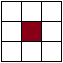
\includegraphics[width=0.3\textwidth]{\ImgPath/rys/elementy_strukturalne/1.png}}
	\subfigure[]
	{\label{fig:b}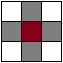
\includegraphics[width=0.3\textwidth]{\ImgPath/rys/elementy_strukturalne/2.png}}
	\subfigure[]
	{\label{fig:b}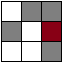
\includegraphics[width=0.3\textwidth]{\ImgPath/rys/elementy_strukturalne/3.png}}
	\caption{Przykładowe elementy strukturalne, gdzie punkt kolorze czerwonym jest punktem centralnym}
\end{figure}

\paragraph{Etapy przekształceń morfologicznych:}
\begin{enumerate}
	\item Szablon strukturalny jest przesuwany po całym obiekcie, tak aby punkt centralny szablonu był analizowanym pikselem
	\item Następuje porównanie otoczenia analizowanego piksela z elementem strukturalnym
	\item W zależności od stosowanej operacji morfologicznej wartość analizowanego piksela zmienia się lub też pozostaje bez zmian
\end{enumerate}

\paragraph{Erozja:}\mbox{} \\
Jest to operacja zwężania i zmniejszania poprzez usunięcie pikseli granicznych. Usuwa wszystkie mniejsze obiekty, które możemy zinterpretować jako szumy. 

\paragraph{Etapy operacji erozji:}
\begin{enumerate}
	\item Element strukturalny przesuwany jest iteracyjnie po całym obiekcie,  tak aby punkt centralny szablonu był analizowanym pikselem
	\item Porównuje się otoczenie analizowanego piksela z elementem strukturalnym
	\item  Jeżeli przynajmniej jeden piksel z otoczenia objętego przez szablon strukturalny ma wartość równą 0, to punkt centralny przyjmuje wartość 0. Jeżeli zaś taki przypadek nie wystąpił piksel centralny zachowuje swoją poprzednią wartość
\end{enumerate}

\begin{figure}[H]
	\centering
	\subfigure[Obraz początkowy]
		{\label{fig:a}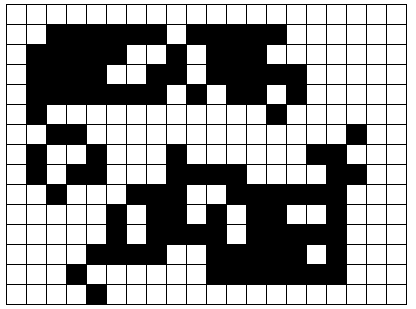
\includegraphics[width=0.3\textwidth]{\ImgPath/rys/operacje_morfologiczne/szablon.png}}
	\subfigure[Element struturalny, punkt czerwony jest punktem centralnym]
		{\label{fig:b}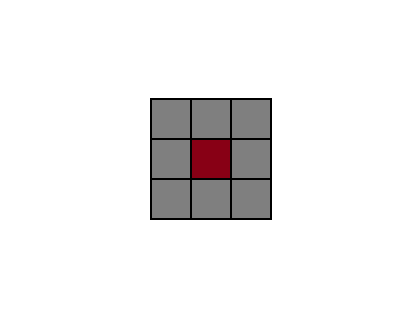
\includegraphics[width=0.3\textwidth]{\ImgPath/rys/operacje_morfologiczne/e.png}}
	\subfigure[Obraz wyjściowy]
		{\label{fig:b}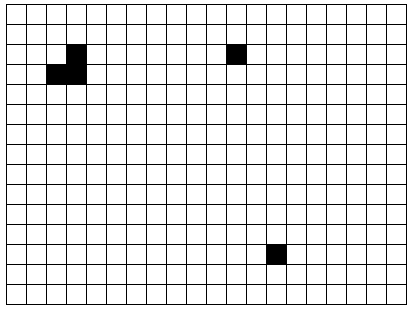
\includegraphics[width=0.3\textwidth]{\ImgPath/rys/operacje_morfologiczne/erozja.png}}
	\caption{Operacja erozji na obrazie binarnym}
\end{figure}

\paragraph{Dylatacja:}\mbox{} \\
Jest to operacja rozszerzania i zwiększania. Pozwala na wypełnienie dziur binarnych w obiektach. Jeżeli dwa obiekty są położone blisko siebie, może nastąpić złączenie w jeden obiekt.

\paragraph{Etapy operacji erozji:}
\begin{enumerate}
	\item Element strukturalny przesuwany jest iteracyjnie po całym obiekcie, tak aby punkt centralny szablonu był analizowanym pikselem
	\item Porównuje się otoczenie analizowanego piksela z elementem strukturalnym
	\item Jeżeli przynajmniej jeden piksel z otoczenia objętego przez szablon strukturalny ma wartość równą 1, to punkt centralny przyjmuje również wartość 1. Jeżeli zaś wszystkie piksele z otoczenia piksela centralnego określonego przez element strukturalny mają wartość 0 to wówczas piksel centralny przyjmuje wartość 0.
\end{enumerate}

\begin{figure}[H]
	\centering
	\subfigure[Obraz początkowy]
	{\label{fig:a}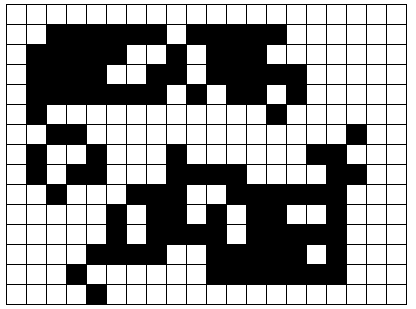
\includegraphics[width=0.3\textwidth]{\ImgPath/rys/operacje_morfologiczne/szablon.png}}
	\subfigure[Element struturalny, punkt czerwony jest punktem centralnym]
	{\label{fig:b}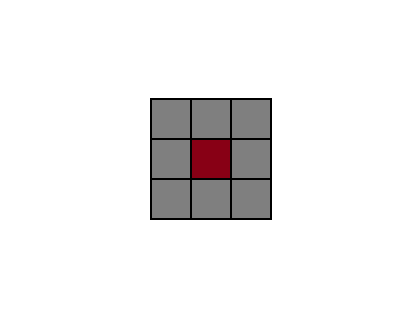
\includegraphics[width=0.3\textwidth]{\ImgPath/rys/operacje_morfologiczne/e.png}}
	\subfigure[Obraz wyjściowy]
	{\label{fig:b}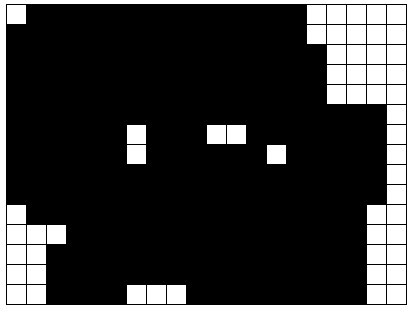
\includegraphics[width=0.3\textwidth]{\ImgPath/rys/operacje_morfologiczne/dylatacja.png}}
	\caption{Operacja dylatacji na obrazie binarnym}
\end{figure}

\paragraph{Otwarcie:}\mbox{} \\
Operacja otwarcia morfologicznego jest definiowana przez połączenie metod erozji oraz dylatacji. Metoda ta wygładza obiekt, usuwa niechciane szumy, a w dodatku nie modyfikuje znacząco wielkości obiektów tak jak to jest w przypadku zastosowania operacji erozji czy dylatacji.

\paragraph{Etapy operacji otwarcia:}
\begin{enumerate}
	\item Wykonywana jest operacja erozji na zadanym obrazie
	\item Wykonywana jest operacja dylatacji na obraz, który jest wynikiem erozji z punktu 1.
\end{enumerate}

\begin{figure}[H]
	\centering
	\subfigure[Obraz początkowy]
	{\label{fig:a}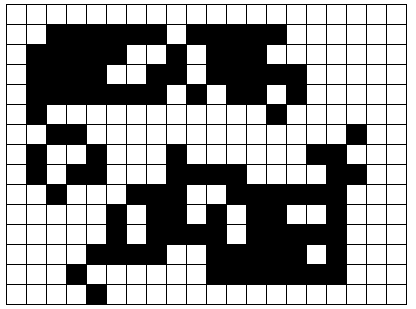
\includegraphics[width=0.3\textwidth]{\ImgPath/rys/operacje_morfologiczne/szablon.png}}
	\subfigure[Element struturalny, punkt czerwony jest punktem centralnym]
	{\label{fig:b}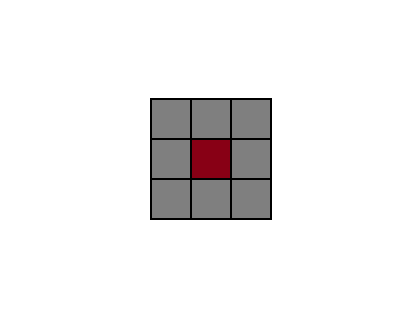
\includegraphics[width=0.3\textwidth]{\ImgPath/rys/operacje_morfologiczne/e.png}}
	\subfigure[Obraz wyjściowy]
	{\label{fig:b}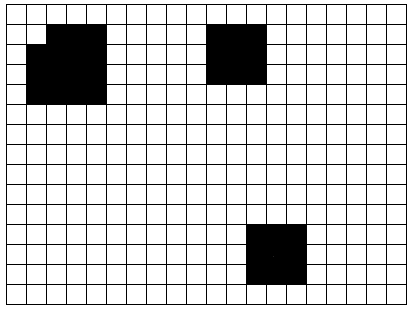
\includegraphics[width=0.3\textwidth]{\ImgPath/rys/operacje_morfologiczne/otwarcie.png}}
	\caption{Operacja otwarcia na obrazie binarnym}
\end{figure}

\paragraph{Zamknięcie:}\mbox{} \\
Operacja zamknięcia łączy w sobie połączenie dwóch metod dylatacji oraz erozji, analogicznie jak było w przypadku operacji zamknięcia, jednakże w odwrotnej kolejności. W rezultacie uzyskujemy połączenie obiektów o zbliżonych odległościach, wypełnienie dziur w obiektach, jednakże końcowy kształt obiektu zostaje w dużym stopniu zmieniony w stosunku do kształtu przed zastosowaniem operacji zamknięcia.

\paragraph{Etapy operacji otwarcia:}
\begin{enumerate}
	\item Wykonywana jest operacja dylatacji na zadanym obrazie
	\item Wykonywana jest operacja erozji na obraz, który jest wynikiem erozji z punktu 1.
\end{enumerate}

\begin{figure}[H]
	\centering
	\subfigure[Obraz początkowy]
	{\label{fig:a}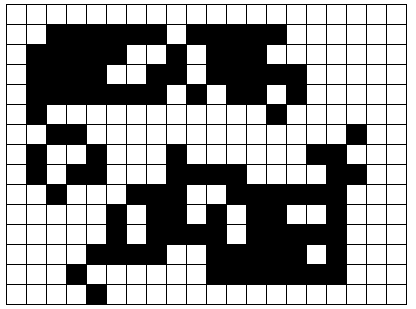
\includegraphics[width=0.3\textwidth]{\ImgPath/rys/operacje_morfologiczne/szablon.png}}
	\subfigure[Element struturalny, punkt czerwony jest punktem centralnym]
	{\label{fig:b}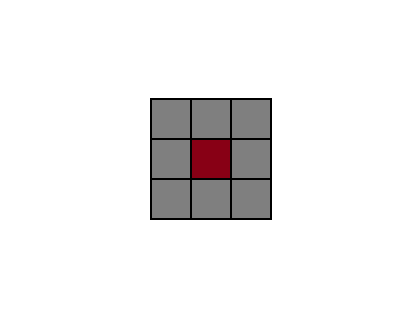
\includegraphics[width=0.3\textwidth]{\ImgPath/rys/operacje_morfologiczne/e.png}}
	\subfigure[Obraz wyjściowy]
	{\label{fig:b}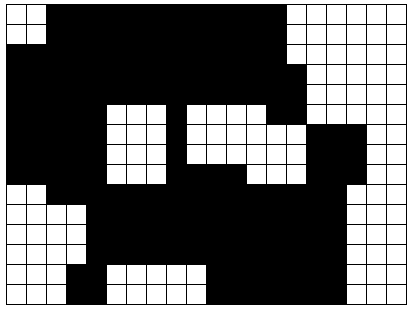
\includegraphics[width=0.3\textwidth]{\ImgPath/rys/operacje_morfologiczne/zamkniecie.png}}
	\caption{Operacja zamknięcia na obrazie binarnym}
\end{figure}

\section{Filtry ruchu}
Filtry ruchu są wykorzystywane do generowania maski binarnej zawierającej poruszające się obiekty. Tak zwany z ang. background subtraction wykorzystuje różnicę z dwóch różnych klatek z pliku wideo. Odejmowanie dwóch klatek pozwala nam prześledzić, które z części obrazów zmieniły się. Różnica dwóch pikseli da nam wartość niezerową, tylko wtedy jeżeli z analizowanych klatkach wartość odpowiadających pikseli różni się, co interpretujemy, że ta część obrazu poruszyła się. 

\begin{figure}[H]
	\centering
	\subfigure[Tło]
	{\label{fig:a}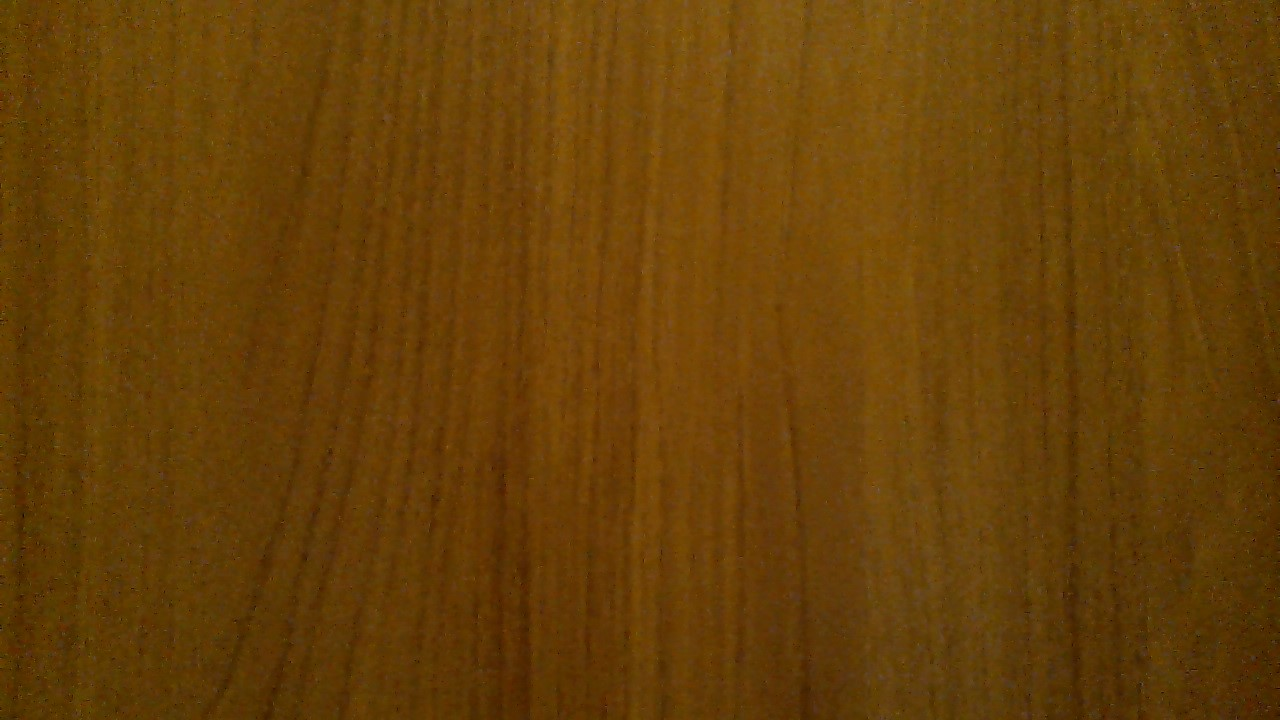
\includegraphics[width=0.3\textwidth]{\ImgPath/rys/bs/tlo.jpg}}
	\subfigure[Zdjęcie]
	{\label{fig:b}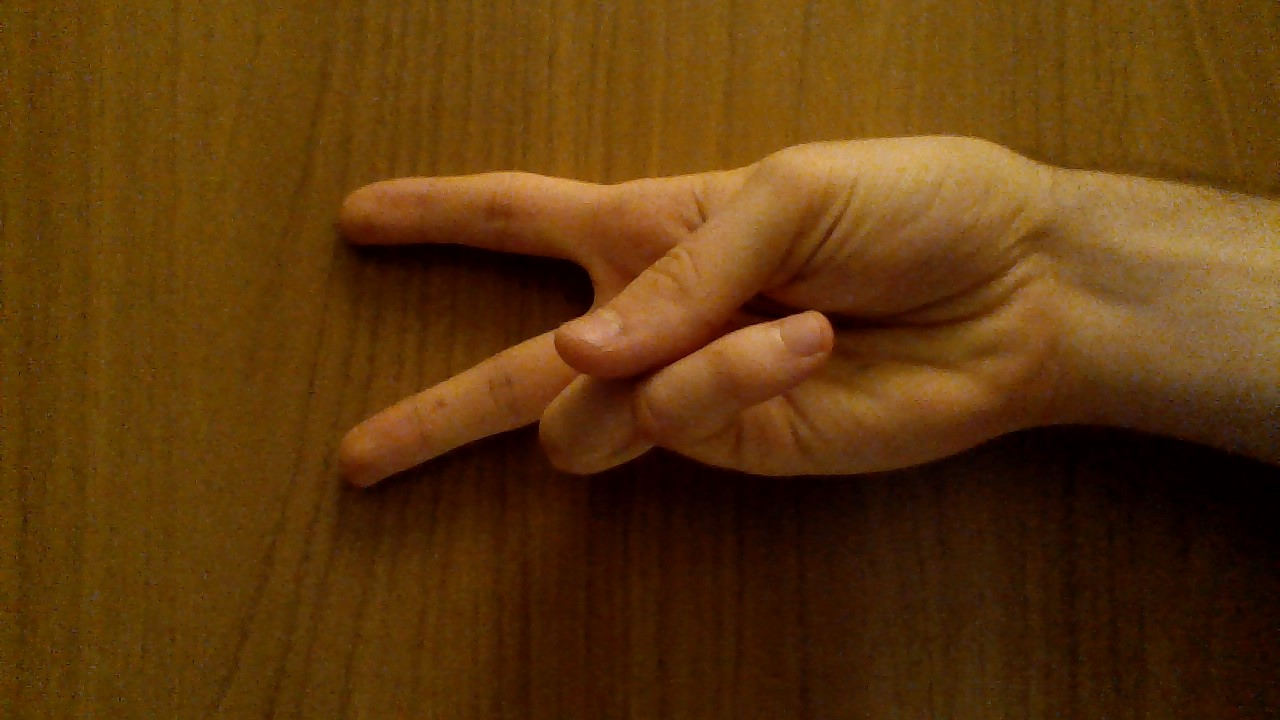
\includegraphics[width=0.3\textwidth]{\ImgPath/rys/bs/img.jpg}}
	\subfigure[Różnica zdjęcia i tła ]
	{\label{fig:b}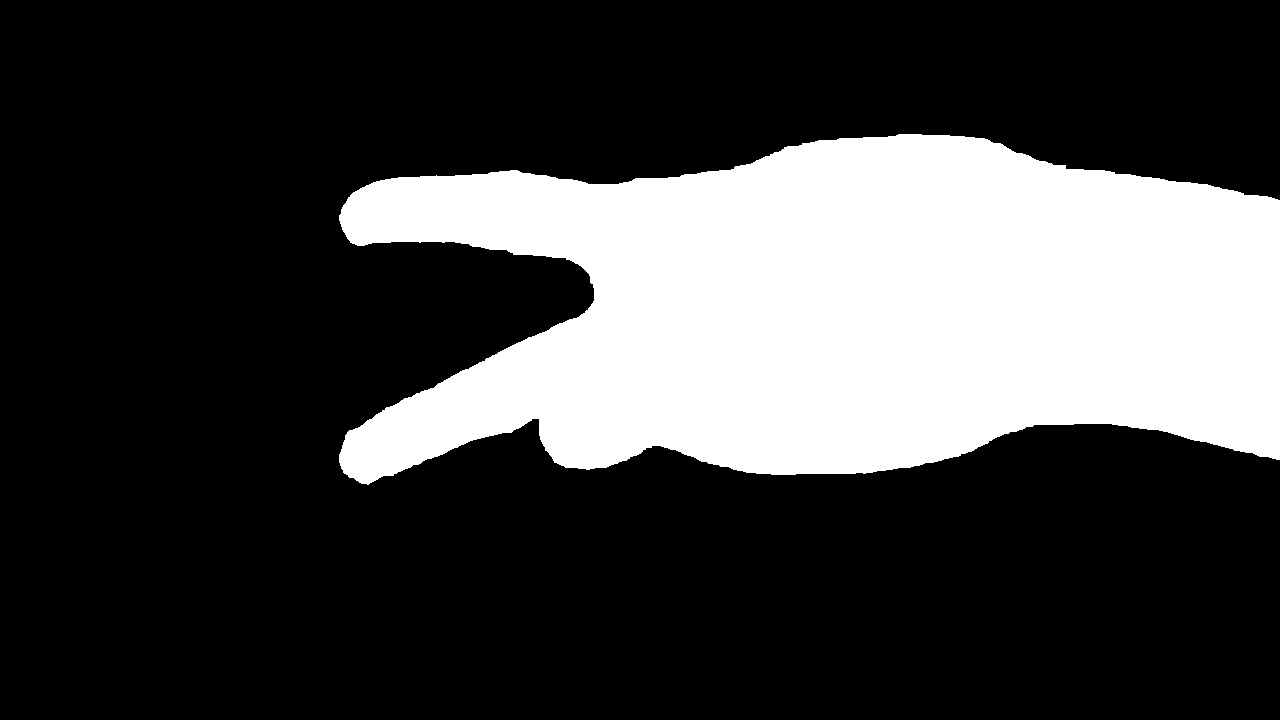
\includegraphics[width=0.3\textwidth]{\ImgPath/rys/bs/bin.jpg}}
	\caption{Przykładowe metody background subtractor z biblioteki OpenCV}
\end{figure}

OpenCV w swojej bibliotece posiada wiele gotowych rozwiązać do wykrywania obiektów w ruchu. Jako jedne z najczęściej wykorzystywanych metod możemy wyróżnić następujące:
\begin{itemize} 
	\item BackgroundSubtractorMOG
	\item BackgroundSubtractorMOG2
	\item BackgroundSubtractorGMG
\end{itemize} 
	
\begin{figure}[H]
	\centering
	\subfigure[BackgroundSubtractorMOG]
	{\label{fig:a}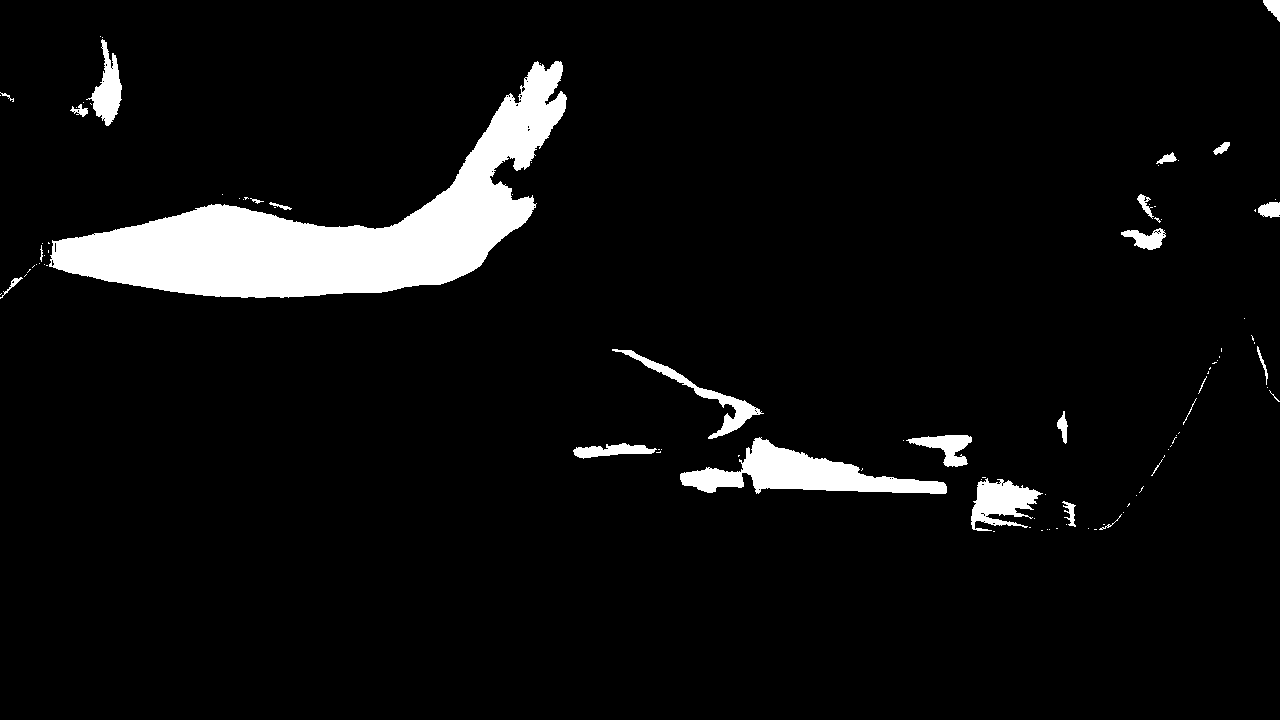
\includegraphics[width=0.3\textwidth]{\ImgPath/rys/bs/mog.png}}
	\subfigure[BackgroundSubtractorMOG2]
	{\label{fig:b}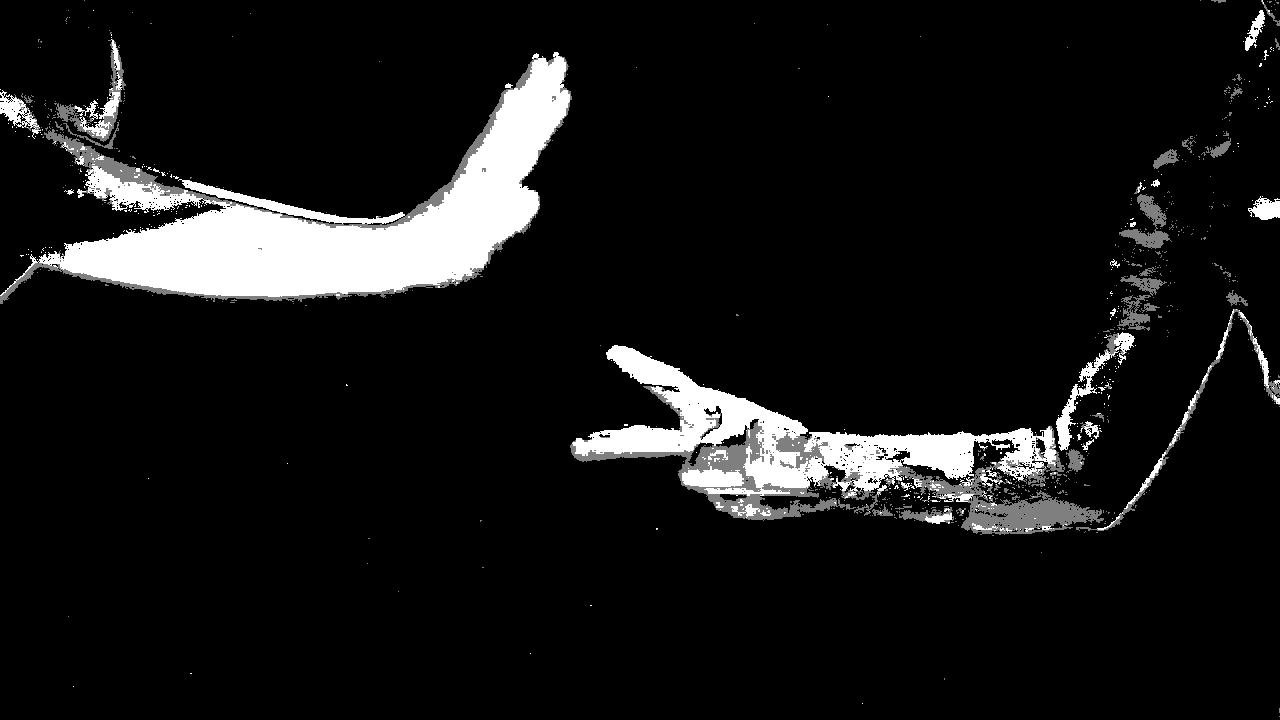
\includegraphics[width=0.3\textwidth]{\ImgPath/rys/bs/mog2.png}}
	\subfigure[BackgroundSubtractorGMG]
	{\label{fig:b}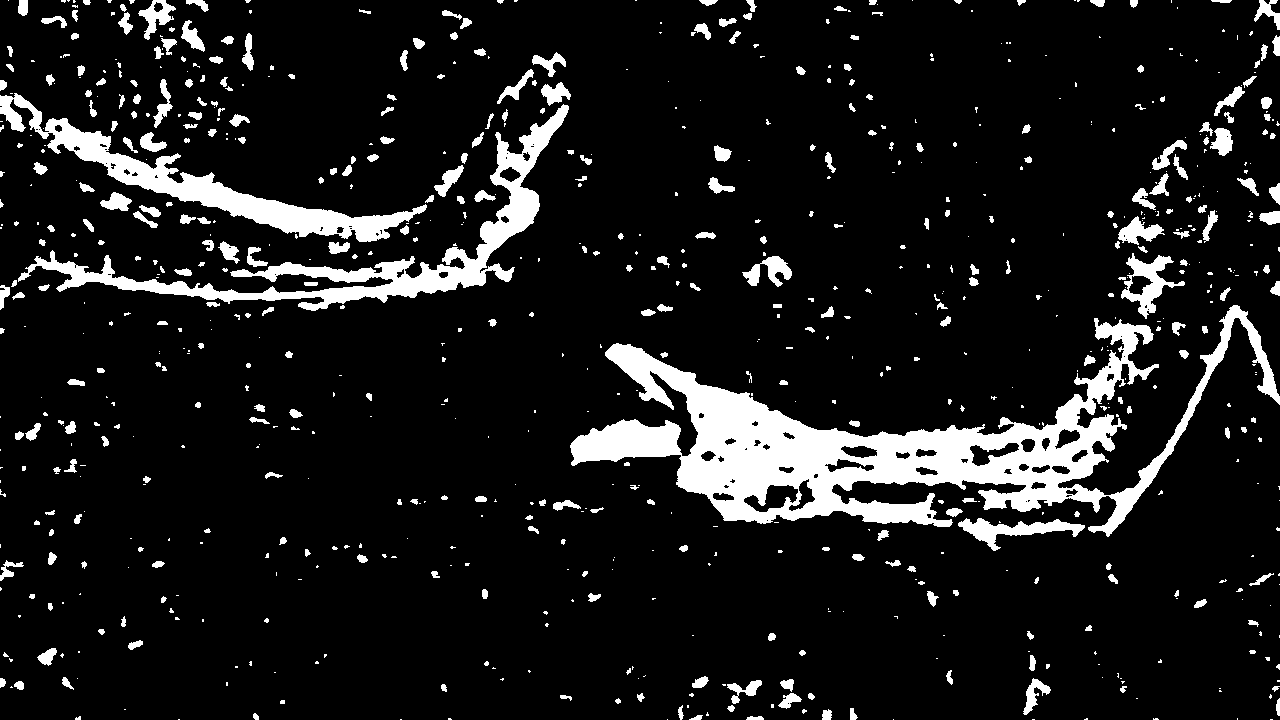
\includegraphics[width=0.3\textwidth]{\ImgPath/rys/bs/gmg.png}}
	\caption{Przykładowe metody background subtractor z biblioteki OpenCV}
\end{figure}

W celu polepszenia efektów, należy pozbyć się niedokładnej segmentacji oraz możliwych szumów,  które mogą wystąpić podczas analizy. Są one spowodowane różnymi odbiciami, cieniami czy innymi niezauważalnymi ruchami. Wówczas należy wykorzystać przedstawione wcześniej operacje morfologiczne, które poprawią nam wykonaną detekcję.

\section{Detekcja kolorów}
Celem detekcji kolorów jest wygenerowanie obrazu binarnego, w którym piksele binarne  o wartości prawdy oznaczają piksele, które na zadanym obrazie są w określonym przedziale kolorów. Jeżeli dany piksel nie należy do określonego  przedziału, wówczas obraz binarny w tym punkcie otrzymuje wartość fałszu. Detekcja taka pozwala na wyłuskania tylko obiektów o określonym koloru.

Detekcja jest bardzo wrażliwa na różnego rodzaju szumy. Częstymi powodem występowanie ich jest zmienne oświetlenie. Obiekt przy różnym świetle możemy odbierać kolorystycznie całkowicie inaczej. W przypadku, kiedy analizujemy dynamiczny ruch, wówczas dynamika również może wpływać na kolorystykę danego obiektu. Te wszystkie czynniki, sprawiają, że detekcja określonego koloru nie jest zadaniem takim prostym. 

Aby polepszyć efekt końcowy detekcji obiektów o określonym kolorze, należy analogicznie jak w przypadku detekcji ruchu, wykorzystać odpowiednie operacje morfologiczne. 

Przy detekcji kolorów tradycyjny model rgb (red, green, blue), najczęściej nie jest wystarczająco dobrym modelem. W zadaniach takich zdecydowanie lepiej sprawuje się model HSV.

\begin{figure}[H]	
	\centering
	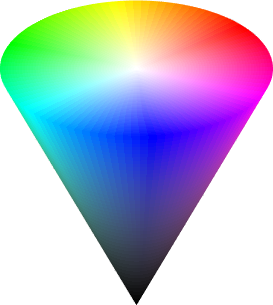
\includegraphics[width=0.4\textwidth]{\ImgPath/rys/hsv.png}
	
	\caption{  \textbf{Model HSV}}
\end{figure}

HSV (ang. Hue Saturation Value) jest to model opisu przestrzeni barw, wprowadzony przez Alveya Raya Smitha w 1978 roku.

Model składa się z następujących części: barwa, nasycenie, wartość. Geometrycznie możemy go przedstawić jako stożek. Wszystkie barwy wywodzą się ze światła białego, czyli ze środka stożka. Składowa H, oznacza barwę w postaci kąta od 0 do 360 stopni. Składowa S czyli nasycenie, geometrycznie to odległość od środka na promieniu podstawy. Decyduje o bliskości naszego koloru do koloru białego. Ostatnia składowa V, to wartość oznaczająca wysokość na stożku, co możemy traktować jako jasność naszego koloru. Czym mniejsza jej wartość tym kolor ciemniejszy.

\chapter{Sztuczna inteligencja}
\section{Sztuczna inteligencja, uczenie maszynowe, głębokie uczenie}
\section{Sieci neuronowe}
\subsection{Uczenie sieci neuronowych}

\section{Klasyfikatory}
Klasyfikacja to wyznaczanie klasy decyzyjnej do której należy nowy, nieznany dotąd obiekt. Metody klasyfikacji możemy podzielić na dwie kategorie. Pierwsza z nich jest  klasyfikacją nadzorowaną, druga zaś to klasyfikacja nienadzorowana. 

Klasyfikacja nadzorowana w momencie uczenia klasyfikatora tzn. podawania zbioru danych treningowych, musi w sobie zawierać etykietę(atrybut decyzyjny), która oznacza do jakiej klasy należy ten konkretny przypadek. Zaś w przypadku klasyfikacji nienadzorowanej atrybutu decyzyjnego nie istnieje.

\subsection{Klasyfikator KNN}
Klasyfikator KNN jest przykładem klasyfikacji nadzorowanej. Zbiór treningowy zawiera w sobie cechy dla klasyfikatora czyli atrybuty oraz atrybut decyzyjny, który określa przynależność do konkretnej klasy. Elementami wejścia dla stworzenia klasyfikatora jest zbiór uczący. Wyjściem jest klasyfikator, który wykorzystujemy do określania atrybutów decyzyjnych nieznanych wcześniej obiektów.

\paragraph{Po utworzeniu klasyfikatora bazującego na zbiorze uczącym, szacowanie atrybutu decyzyjnego odbywa się w następujących krokach: }
\begin{enumerate}
	\item Ustalamy wartość k
	\item Znajdujemy k obiektów treningowych, najbliższych naszemu obiektowi
	\item Analizowany obiekt należy do klasy najliczniejszej w znalezionym zbiorze z podpunktu 2
\end{enumerate}
	
Ocenianie odległości pomiędzy dwoma obiektami polega na umieszczaniu obiektów w przestrzeni d-wymiarowej, gdzie d opisuje ilość atrybutów dla obiektów. Metryka miary może odbywać się w różny sposób. Najczęściej jest to miara euklidesowa, jednakże możemy również wykorzystać inne miary tj. Manhattana czy Minkowskiego. 

Po znalezieniu k-najbliższych sąsiadów, atrybut decyzyjny przyjmuje wartość od najbardziej licznej klasy w wyznaczonym zbiorze.

Rysunek:


\subsection{Dobór i ocena cech}

\section{Python}
Jest to interpretowany, obiektowy język wysokiego poziomu. Używany jest w szerokiej gamie  aplikacjach. Jest językiem ogólnego przeznaczenia, co oznacza, że może zostać wykorzystany praktycznie do wszystkiego. Jest rozwijany jako projekt otwartoźródłowy. Pojawił się w roku 1991, zaprojektowany przez holenderskiego programistę Guido van Rossum.

\paragraph{Zalety używania Pythona:}
\begin{itemize} 
	\item prosta, czytelna, klarowna składnia, zmniejszająca ilość potrzebnych linijek kodu w programach
	\item dynamicznie zarządza pamięcią oraz typy danych
	\item nie wymusza stylu programowania
	\item jest wieloplatformowy
	\item posiada bogaty zbiór różnego rodzaju bibliotek
	\item łatwy do nauczenia, nawet dla osób zaczynających programować
	\item szybkość działania w stosunku do innych języków kryptowych
\end{itemize} 
\mbox{} \\
Jeśli mielibyśmy dyskutować o wadach językach Python to ciężko jednoznacznie wskazać takie. Na pewno część z programistów może uznać zalety dynamicznego zarządzania typami jako wadę, ponieważ w niektórych przypadkach może spowodować błędy trudniejsze do znalezienia. Działania Pythona jest również wolniejsze w stosunku do języków takich jak C czy C++.  Za jedną z wad na pewno można uznać sposób programowania obiektowego jakie odbywa się w Pythonie. W szczególności nie ma enkapsulacji, istnieją metody które symulują takie działa, jednakże w stosunku do innych języków  obiektowych czytelność kodu zdecydowanie jest zmniejszona.

Język mimo swoich lat ciągle zyskuje na popularności. Ostatnio wszedł do pierwszej trójki najbardziej popularnych języków programowania według TIOBE (stan na grudzień 2018), wyprzedzając między innymi język C++, a ulegając jedynie językowi Java oraz C. Wzrost języka Python na pewno można łączyć ze wzrostem popularności uczenia maszynowego i głębokich sieci, gdzie język Python jest jednym z najlepszych, jak nie najlepszym językiem w tych dziedzinach. Bardzo bogata biblioteka oraz przyjemna składnie sprawia, że język Python jest częściej wykorzystywany.  

Jako ciekawostkę można powiedzieć, że nazwa języka Python wzięła się nie od zwierzęcia, lecz od słynnego Brytyjskiego serialu "Monty Python’s Flying Circus".

\section{TensorFlow}
Jest to biblioteka programistyczna wykorzystywana w uczeniu maszynowym i głębokich sieciach neuronowych. Została wydana jako otwarte oprogramowanie przez Google Brain Team w dniu 9 listopada 2015.

Umożliwia pisanie programów m.in. w językach takich jak Python czy C. Jest dostępny na 64-bitowych systemach operacyjnych: Windows, Linux, macOS oraz na platformach mobilnych: Android oraz iOS. Zaś w maju 2017 został wydany TensorFlow Lite jako dedykowane rozwiązanie specjalnie dla użytkowników Androida.

Olbrzymią zaletą TensorFlow jest to, że reprezentuje on paradygmat Dataflow, w którym program ma postać grafu skierowanego modelującego przepływ danych pomiędzy niezależnymi operacjami w węzłach. W pierwszym kroku należy zdefiniować model, a następnie stworzyć tzw. TensorFlow session, która pozwala na uruchomienie programu. Takie podejście do pisania programów posiada ogromną zaletą jaką jest możliwość efektywnego programowania równoległego oraz rozproszonego. 

TensorFlow daje możliwość nie tylko wykorzystania CPU, ale równie dobrze korzystania z GPU. Wszystko to powoduje pełne wykorzystanie mocy obliczeniowej komputerów przy obliczeniach równoległych.

TensorFlow oprócz niskopoziomowych struktur posiada również moduły wyższego poziomu. Do modułów niskiego poziomu możemy odwoływać się poprzez warstwę API, która umożliwia łatwy do używania interfejs przeznaczony do modelów głębokiego uczenia. Zaś nad warstwą API znajduje się warstwa wysokiego poziomu, przykładem jej jest Keras.

\section{Keras}
Otwartoźródłowa biblioteka programistyczna napisana w języku Python wydana w dniu 27 marca 2015 napisana przez pierwotnego autora François Chollet. 

Jej głównym przeznaczeniem jest to, aby w jak najprostszy i  jak najszybszy sposób umożliwić pracę w głębokich sieciach neuronowych. Co więcej, biblioteka została zaprojektowana w sposób przyjemny do użytkowania, skupiona na modularności oraz rozszerzalności. Zaś od 2017 roku TensorFlow wspiera w swojej bibliotece Kerasa. Dzięki czemu Keras jest wysokopoziomową warstwą tworzenia modelów sieci neuronowych i jej uczenia.

\chapter{Gra papier, kamień, nożyce}
Jest to klasyczna gra towarzyska, w tradycyjnym wariancie przeznaczona dla dwóch graczy. W każdej rundzie każdy z graczy pokazuje gest przez siebie wybrany z trzech dostępnych. Wszystkie rundy odbywają się na ustalony wcześniej sygnał, a pokazywane gesty powinny być jak najbardziej zsynchronizowane. Gra kończy się wtedy, jeżeli jeden z graczy osiągnie określoną wcześniej ilość zwycięstw.


\paragraph{Trzy gesty dozwolone w grze:}
\begin{itemize} 
	\item Papier
	\item Kamień
	\item Nożyce
\end{itemize} 

\begin{figure}[H]
	\centering
	\subfigure[Gest papieru]
	{\label{fig:a}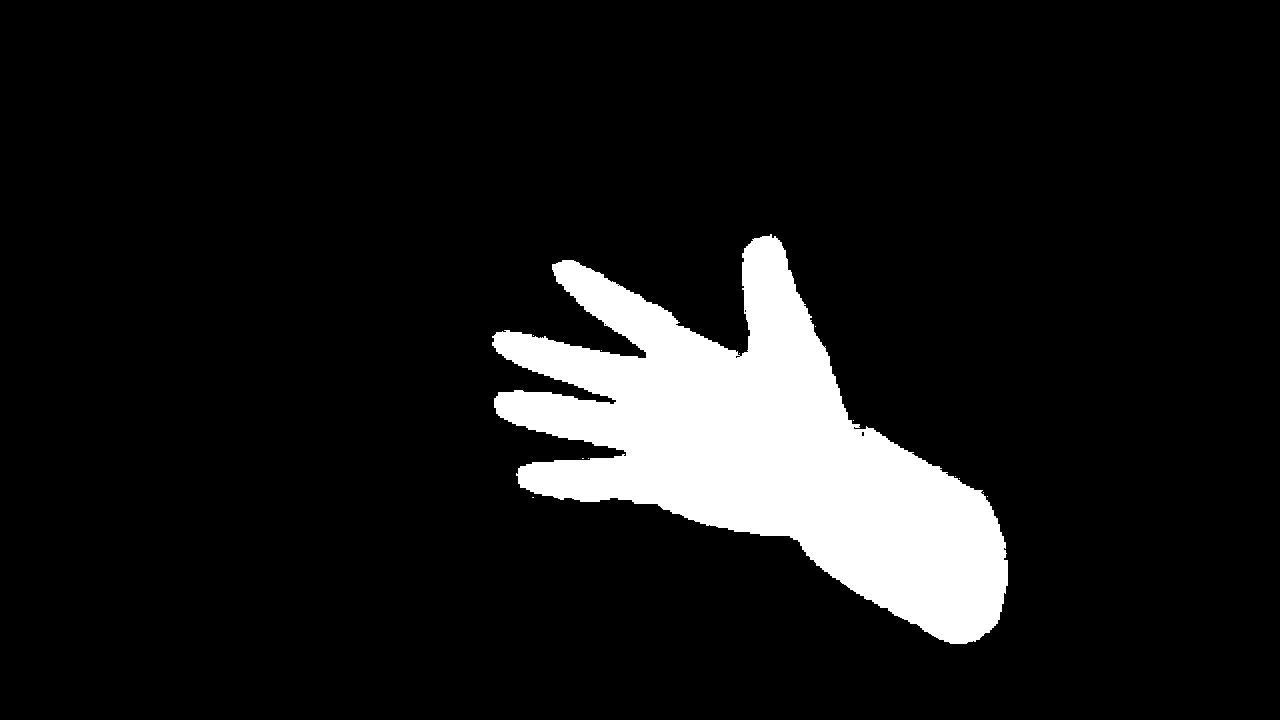
\includegraphics[width=0.3\textwidth]{\ImgPath/rys/gesty_gry/papier.png}}
	\subfigure[Gest kamienia]
	{\label{fig:b}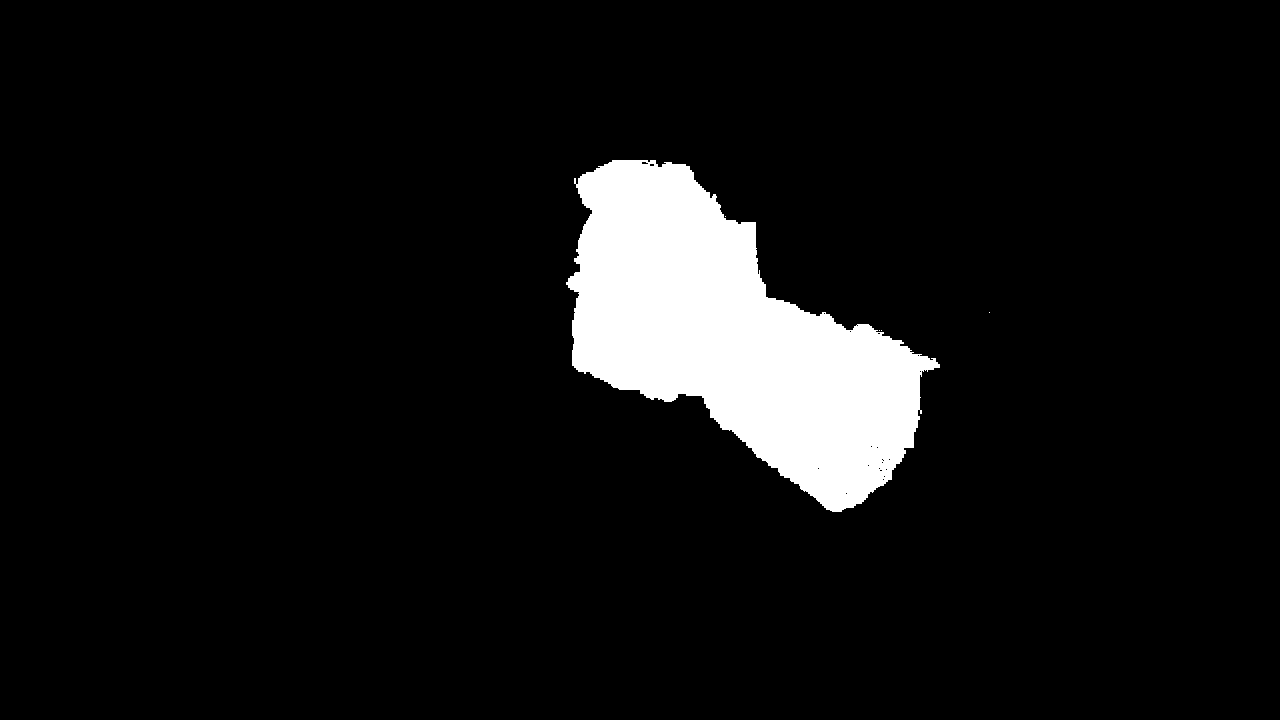
\includegraphics[width=0.3\textwidth]{\ImgPath/rys/gesty_gry/kamien.png}}
	\subfigure[Gest nożyc]
	{\label{fig:b}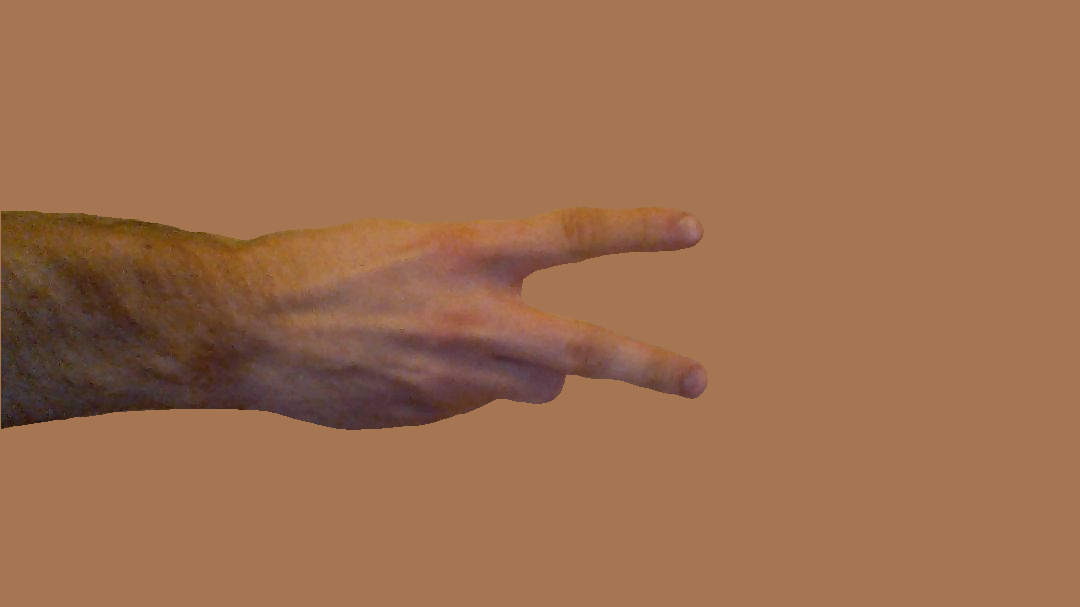
\includegraphics[width=0.3\textwidth]{\ImgPath/rys/gesty_gry/nozyce.png}}
	\caption{BackgroundSubtractorKNN na gestach z gry papier, kamier, nożyce}
\end{figure}

Zwycięzca określany jest w zależności od kombinacji gestów pokazanych przez graczy. Jeżeli oba gracze pokazali ten sam gest, wówczas następuje remis. 

\paragraph{W przypadku kombinacji:}
\begin{itemize} 
\item papier-kamień - zwycięzcą zostaje gracz, który pokazał gest papieru
\item papier-nożyce - zwycięzcą zostaje gracz, który pokazał gest nożyc
\item kamień-nożyce - zwycięzcą zostaje gracz, który pokazał gest kamienia
\end{itemize} 
\mbox{} \\	
Zachowując takie zasady, każdy z gestów ma takie samo prawdopodobieństwo zwycięstwa. W grze liczy się w dużej mierze szczęście, ale także umiejętność przewidywania gestów przeciwnika.

\chapter{Rozpoznawanie gestów w grze papier, kamień, nożyce}
\section{Aktywizacja danych}
Pierwszym etapem mojej pracy była aktywizacja danych potrzebnych do uczenia maszynowego. Zbieranie danych polegało na nagrywaniu plików wideo na których dana osoba wykonywała określony gest. W swojej pracy dyplomowej zakładam, że każdy wykonywany gest, jest wykonany w niebieskiej rękawiczce. Takie założenie będę zakładał w całej swojej pracy inżynierskiej.
\begin{figure}[H]	
	\centering
	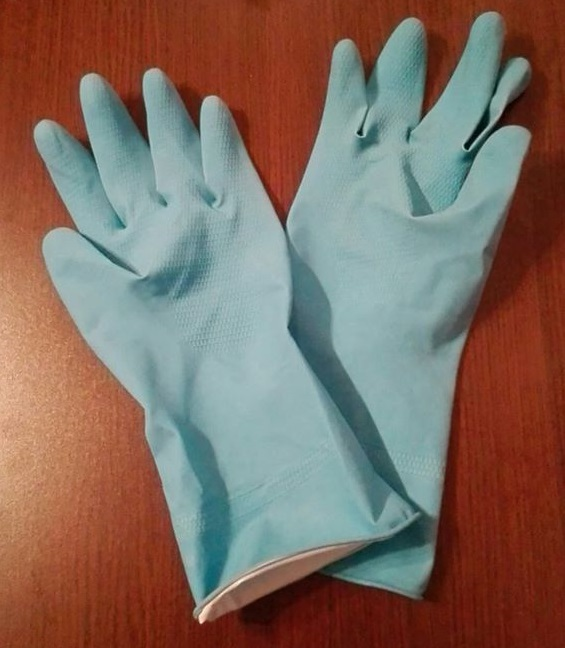
\includegraphics[width=0.4\textwidth]{\ImgPath/rys/rekawiczki.jpg}
	
	\caption{  Rękawiczki wykorzystywane w pracy inżynierskiej}
\end{figure}

\paragraph{Do nagrywania plików używałem dwóch kamer dedykowanych w laptopach:}
\begin{itemize}
	\item USB2.0 UVC HD Webcam
	\item HD Webcam
\end{itemize}
\mbox{} \\
\noindent
Obie kamery pozwoliły na zadowalające efekty zbierania danych. Jakość zdjęć przy dostatecznie dobrym oświetleniu była bardzo zadowalające, pozwalające bez problem rozpoznawać wykonywany gest. Również ilość klatek na sekundę, pozwoliła, aby dynamiczny ruch był płynny i móc go pomyślnie wysegmentować.

W celu zebrania jak najszerszego zakres danych, zbieranie gestów nie ograniczyło się do jednej osoby, jednakże do pięciu różnych osób:
\begin{itemize}
	\item trzech kobiet
	\item dwóch mężczyzn
\end{itemize}
\mbox{} \\
Zbieranie danych na różnych osobach pozwala na zmniejszani wpływu charakterystycznych cech dla danej osoby:
\begin{itemize}
	\item długości dłoni
	\item szerokości dłoni
	\item ułożenia palców
\end{itemize}
\mbox{} \\
Po zgromadzeniu całego materiału wideo przeszedłem do etapu wyznaczania numerów klatek filmu na których był moment wykonanego gestu. Klatki te będę wykorzystywał w późniejszym  etapie segmentacji dłoni z wykonanym gestem.

Tak zebrane danych daje ogólny pogląd na różnorodność cech danego gestu. Sprawia, że uczenie maszynowe jest skuteczne i daje oczekiwane rezultaty. Aby zapewnić prawidłowe rozpoznawanie, należy zgromadzić sporą ilość gestów. 

\paragraph{W mojej pracy inżynierskiej wykorzystywałem zbiór danych składający się z:}
\begin{itemize}
	\item 300 próbek gestu papieru
	\item 300 próbek gestu kamienia
	\item 300 próbek gestu nożyc
\end{itemize}



\section{Detekcja ruchu}
Po zebraniu danych zająłem się ich przetwarzaniem. Pierwszym krokiem było wysegmentowanie obiektów, które znajdowały się w ruchu. Aby to osiągnąć należało wygenerować maskę binarną, którą rozdzielała tło od obiektów pierwszoplanowych. Do tego wykorzystałem tzw. background subtraction czyli tłumacząc z angielskiego ,,odejmowanie tła''.

Metodę dokładną z jakiej skorzystałem była to funkcja z biblioteki OpenCV BackgroundSubtractorKNN. Moim zdaniem uważam że w przypadkach na jakich testowałem segmentację ruchu, metoda ta dawała najlepsze rezultaty w porównaniu z innymi dostępnymi w bibliotece OpenCV. 

Metoda ta pozwoliła uzyskać następujące efekty:


Można zauważyć, że wykonywany ruch dłonią jest bardzo widoczny, jednakże dodatkowa zawarta jest duża ilość szumy, który w późniejszym czasie należy się pozbyć.
\begin{figure}[H]
	\centering
	\subfigure[Gest papieru]
	{\label{fig:a}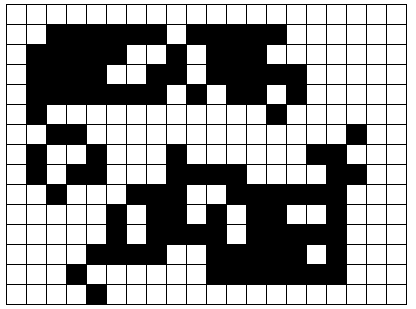
\includegraphics[width=0.3\textwidth]{\ImgPath/rys/operacje_morfologiczne/szablon.png}}
	\subfigure[Gest kamienia]
	{\label{fig:b}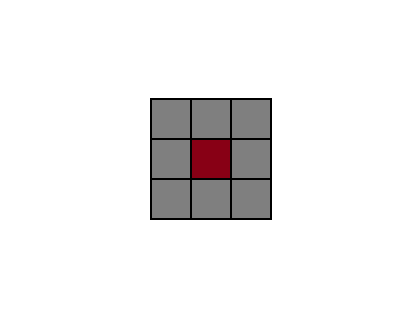
\includegraphics[width=0.3\textwidth]{\ImgPath/rys/operacje_morfologiczne/e.png}}
	\subfigure[Gest nożyc]
	{\label{fig:b}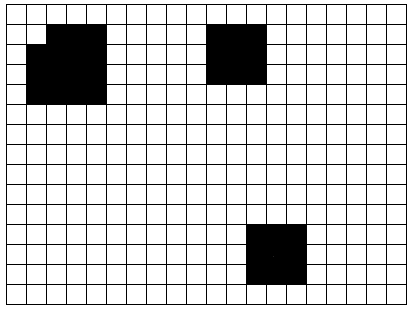
\includegraphics[width=0.3\textwidth]{\ImgPath/rys/operacje_morfologiczne/otwarcie.png}}
	\caption{BackgroundSubtractorKNN na gestach z gry papier, kamier, nożyce}
\end{figure}

\section{Detekcja kolorów}
Równolegle do segmentacji obiektów w ruchu, zająłem się segmentacją obiektów o określonym kolorze. W swojej pracy dyplomowej założyłem, że każdy wykonywany gest jest pokazywany w niebieskiej rękawiczce, w celu łatwiejszej segmentacji dłoni. Nie użyłem tradycyjnego koloru skóry dla osób wschodnio-europejskich ze względu na fakt, że oprócz segmentacji dłoni można było wysegmentować również pozostałe części ręki, jak również inne części ciała jak głowy czy klatka piersiowa. A wszystko to mogło spowodować mniej precyzyjne rozpoznanie gestu.

Wybrałem kolor niebieski ze względu na kolor dobrze rozróżniający się od innych, na który nie wpływa aż tak znacząco moc oświetlenia, który może wpłynąć negatywnie na rozpoznawany kolor.

\section{Szumy w zbiorze danych}
Połączenie segmentacji obiektów w ruchu oraz obiektów o określonym kolorze niesie za sobą możliwy szum, który dla lepszych efektów rozpoznawania obiektów należy zminimalizować. 

Segmentacja elementów obrazu w ruchu, może nieść ze sobą czum spowodowany tym, że inne obiekty, różne od naszej dłoni też mogą się przesuwać. 
\section{Znajdowanie obiektów}

\section{Dobór i ocena cech}
Po wysegmentowaniu gestów dla uczenia maszynowego nadszedł czas, aby zgromadzony materiał opisać dobranymi cechami. Zbiór danych to wysegmentowana dłoń. Zdecydowałem się, że gesty będę opisywał w następujący sposób.

Przy ocenie jakości dobranych cech w pierwszej kolejności wykorzystałem odchylenie standardowe. Dzięki czemu miałem porównanie jak dana cecha wpływa na określony gest. 

Kolejnym etapie było skuteczności wybranej cechy przy rozpoznawaniu konkretnych dwóch gestów. Do tego wykorzystałem wyt	`odę...

Po wyżej wymienionej ocenie ustaliłem następujące cechy dla danego gestu:


\section{Rozpoznawanie gestów przy pomocy klasyfikatora KNN}

\section{Rozpoznawanie gestów przy pomocy sieci neuronowej}
\subsection{Sieć neuronowa dla cech}
\subsection{Sieć neuronowa obrazów binarnych}
\chapter{Podsumowanie}





\appendix



\begin{thebibliography}{99}


\end{thebibliography}


\end{document}
